\section{研究串联电路}\label{sec:8-12}

在实际的电路里,通常都连着几个或者更多的导体,它们可能串联着,也可能并联着。
几个导体串联或者并联时,各个导体的电流、电压或电阻跟电路的总电流、总电压或总电阻有什么关系呢?
这些关系在解决电路问题时是经常要用到的。
这一节我们研究导体串联时的关系,下一节我们研究导体并联时的关系。

在 “\hyperref[sec:8-2]{用安培表测电流强度}” 和 “\hyperref[sec:8-4]{用伏特表测电压}” 的实验里,
我们已经知道

\textbf{串联电路中各处的电流强度相等};

\textbf{串联电路两端的总电压等于各部分电路两端的电压之和}。

\begin{wrapfigure}[14]{r}{7cm}
    \centering
    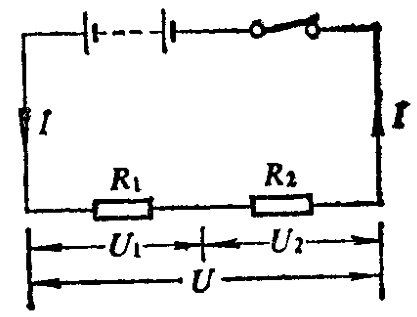
\includegraphics[width=6cm]{../pic/czwl2-ch8-27}
    \caption{}\label{fig:8-27}
\end{wrapfigure}

还有一个重要的问题是,几个导体串联起来,整个串联电路的总电阻是多少呢?

利用欧姆定律很容易解决这个问题。
设串联导体的阻值依次为 $R_1$、$R_2$,串联电路的总电阻为 $R$(图 \ref{fig:8-27})。
那么,由于
$$ U = IR,\quad U_1 = IR_1,\quad U_2 = IR_2 \;\juhao $$

把上列各式代入 $U = U_1 + U_2$ 中,得到
$$ IR = IR_1 + IR_2 \,\text{,} $$
所以 $R = R_1 + R_2$。
这表明\textbf{串联电路的总电阻,等于各串联导体的电阻之和}。

把几个导体串联起来,总电阻比任何一个导体的电阻都大,这是因为导体串联起来就相当于增加了导体的长度。

\liti 把一个 4 欧姆的电阻和一个 6 欧姆的电阻串联起来,接在电压是 12 伏特的电源上。
求这个串联电路中的电流强度。

\begin{enhancedline}
画出电路图(图 \ref{fig:8-28}),注上物理量的符号、数值。
先求出 $R_1$、$R_2$ 串联后的总电阻 $R$,再根据欧姆定律 $I = \dfrac{U}{R}$ 就可以求出电路中的电流强度 $I$。

解: $\begin{aligned}[t]
    &R = R_1 + R_2 = 4\oumu + 6\oumu = 10\oumu \;\juhao \\
    &I = \dfrac{U}{R} = \dfrac{12\fute}{10\oumu} = 1.2\anpei \;\juhao
\end{aligned}$

答:这个串联电路中的电流强度是 1.2 安培。
\end{enhancedline}

\begin{figure}[htbp]
    \centering
    \begin{minipage}{7cm}
    \centering
    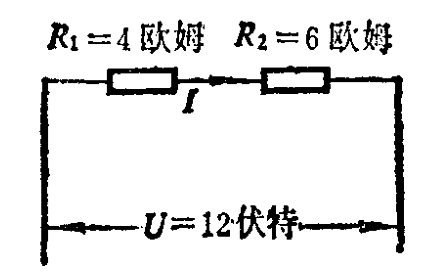
\includegraphics[width=6cm]{../pic/czwl2-ch8-28}
    \caption{}\label{fig:8-28}
    \end{minipage}
    \qquad
    \begin{minipage}{7cm}
    \centering
    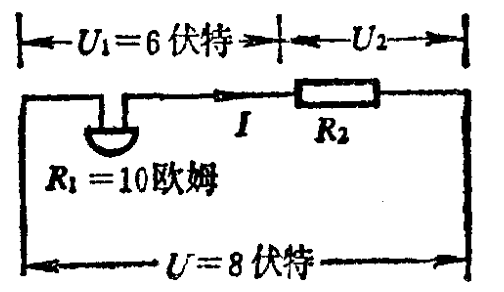
\includegraphics[width=6cm]{../pic/czwl2-ch8-29}
    \caption{}\label{fig:8-29}
    \end{minipage}
\end{figure}

\liti 有一个电铃,它的电阻是 10 欧姆,在正常工作时它两端的电压应该是 6 伏特。
但是我们手边现有的电源电压是 8 伏特,要把电铃接在这个电源上,需要给它串联一个多大的电阻?

画出电路图(图 \ref{fig:8-29})。已知电源电压 $U = 8$ 伏特。
在电路中串联一个电阻 $R_2$,是要用它分去一部分电压,使电铃上的电压为规定值 $U_1 = 6$ 伏特。
所以串联电阻 $R_2$ 上的电压 $U_2$ 应该等于 $U - U_1$。
$R_2$ 的阻值应该多大,才能使它两端的电压为 $U_2$ 呢?
根据欧姆定律,如果知道了通过 $R_2$ 的电流 $I$,就可以求出 $R_2$ 的阻值了。
电铃和电阻 $R_2$ 是串联的,通过它们的电流强度相等。
求出通过电铃的电流,就得到通过 $R_2$ 的电流。
电铃上的电压和它的阻值都是知道的,利用欧姆定律可以求出通过电铃的电流 $I$。
解题的步骤如下。

\begin{enhancedline}
解:$\begin{aligned}[t]
    &U_2 = U - U_1 = 8\fute - 6\fute = 2\fute \,\text{,} \\
    &I = \dfrac{U_1}{R_1} = \dfrac{6\fute}{10\oumu} = 0.6\anpei \,\text{,}
\end{aligned}$

所以 $R_2 = \dfrac{U_2}{I} = \dfrac{2\fute}{0.6\anpei} \approx 3.3\oumu$。

答:需要给电铃串联一个 3.3 欧姆的电阻。
\end{enhancedline}

这是一道比较复杂的物理题。希望同学们用心掌握解题的思路,这对提高你们分析和解决实际问题的能力作用很大。


\lianxi

(1) 图 \ref{fig:8-30} 是手电筒的剖面图和电路图。
\tc{1} 电筒小灯泡正常发光时灯丝的电阻约 10 欧姆,而连接导线(手电筒的金属壳)不过百分之几欧姆。
流过灯丝的电流强度大,还是流过连接导线的电流强度大?
\tc{2} 从干电池组正极出来的电流,是逐渐减小,到负极时减小到零呢,还是在电路的任何部分都一样大呢?

\begin{figure}[htbp]
    \centering
    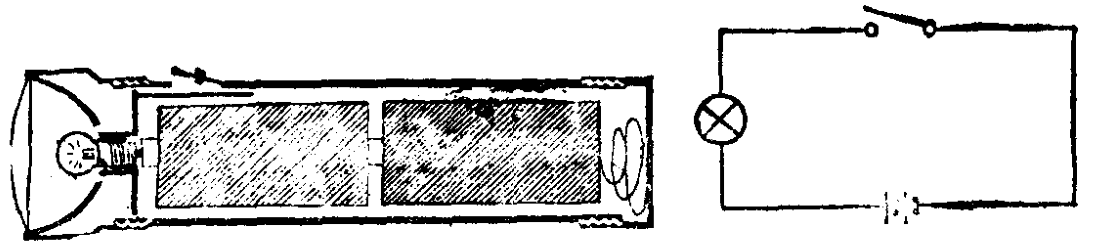
\includegraphics[width=0.7\textwidth]{../pic/czwl2-ch8-30}
    \caption{}\label{fig:8-30}
\end{figure}

(2) 一根铜导线和一根镍铬合金线,长短粗细都相等,把它们串联在电路里,
哪根导线上的电压大?哪根导线中的电流强度大?为什么?

(3) 在图 \ref{fig:8-31} 的电路里,伏特表的示数是 4 伏特,灯泡 $L$ 两端的电压是 3 伏特,求变阻器 $R$ 上的电压。

\begin{figure}[htbp]
    \centering
    \begin{minipage}{7cm}
    \centering
    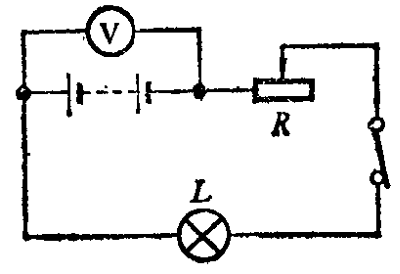
\includegraphics[width=6cm]{../pic/czwl2-ch8-31}
    \caption{}\label{fig:8-31}
    \end{minipage}
    \qquad
    \begin{minipage}{7cm}
    \centering
    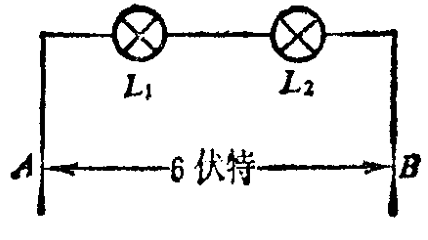
\includegraphics[width=6cm]{../pic/czwl2-ch8-32}
    \caption{}\label{fig:8-32}
    \end{minipage}
\end{figure}

(4) 两盏电灯串联在照明电路里,如果它们的电阻 $R_1$、$R_2$ 分别是 440 欧姆和 110 欧姆,
求这段电路的总电阻,每盏灯里的电流强度,每盏灯两端的电压。

(5) 把电阻分别是 $R_1 = 5$ 欧姆、$R_2 = 10$ 欧姆的两个导体串联起来,然接在电压是 15 伏特的电路里。
求每个导体上的电压。

(6) 在图 \ref{fig:8-32} 所示的电路中,$A$、$B$ 两点的电压是 6 伏特,灯泡 $L_1$ 的电阻是 8 欧姆,
$L_2$ 两端的电压是 4 伏特,求 $L_1$ 中的电流强度。

(7) 在图 \ref{fig:8-31} 的电路里,如果 $L$ 的电阻是 10 欧姆,要使整个电路的电阻是 20 欧姆,
那么变阻器 $R$ 连入电路的电阻应该多大?如果伏特表的示数仍为 4 伏特,这时电路中的电流强度多大?
$L$、$R$ 上的电压各是多大?

(8) 有一个电阻值已看不清楚的电阻器 $R_1$,我们想要测出它的电阻值。
但手边只有一个电池组、一个伏特表、一个电阻值看得清楚的电阻器 $R_2$ 和几根导线。
你有办法测出那个 $R_1$ 的电阻值吗?说出你的办法和理由。

